\documentclass[aspectratio=169,13pt,t] {beamer}
%
% Choose how your presentation looks.
%
% For more themes, color themes and font themes, see:
% http://deic.uab.es/~iblanes/beamer_gallery/index_by_theme.html
%
\mode<presentation>
{
  \usetheme{Madrid}      % or try Darmstadt, Madrid, Warsaw, ...
  \usecolortheme{beaver} % or try albatross, beaver, crane, ...
  \usefonttheme{serif}  % or try serif, structurebold, ...
%  \setbeamertemplate{navigation symbols}{}
  \setbeamertemplate{caption}[numbered]
  \setbeamertemplate{items}[default]
}

\usepackage[,UTF8,linespread=1.2]{ctex}
\usepackage{wrapfig}
\usepackage{caption}
\captionsetup[figure]{name=图,labelsep=period}
\usepackage[,most]{tcolorbox}
\usepackage{picinpar}
\usetikzlibrary{intersections,calc}

\usepackage{xcolor}
\definecolor{xy_blue}{cmyk}{0.6,0.35,0.0,0.4}
\definecolor{xy_orange}{cmyk}{0.0,0.7,1.0,0.0}
\definecolor{xy_green}{cmyk}{0.2,0.0,1.0,0.15}
\xdefinecolor{xy_gold}{RGB}{135,103,79}
\xdefinecolor{xy2_gold}{cmyk}{0,0.35,0.75,0.05}


\setbeamercolor{section number projected}{fg=red,bg=red!20}%控制球的颜色
\setbeamercolor{subsection number projected}{fg=blue,bg=blue!40}
\setbeamercolor{item}{fg=xy_gold} %设置列表项颜色

\usepackage{amsthm}
\newtheorem{peroration}{结论：}
\newtheorem{exploration}{探究：}
\newtheorem{prooft}{证明：}
\newtheorem{question}{问题}
\newtheorem*{solve}{解:}
\newtheorem{instance}{例}   % 解：独立计数器
\BeforeBeginEnvironment{peroration}{%
	\setbeamercolor{block title}{bg=xy_green,fg=white}
	\setbeamercolor{block body}{bg=xy_green!10}
}
\AfterEndEnvironment{peroration}{
	\setbeamercolor{block title}{bg=xy_blue,fg=white}
	\setbeamercolor{block body}{bg=xy_blue!10}
}
\BeforeBeginEnvironment{exploration}{%
	\setbeamercolor{block title}{bg=xy_orange,fg=white}
	\setbeamercolor{block body}{bg=xy_orange!10}
}
\AfterEndEnvironment{peroration}{
	\setbeamercolor{block title}{bg=xy_blue,fg=white}
	\setbeamercolor{block body}{bg=xy_blue!10}
}
\BeforeBeginEnvironment{solution}{%
	\setbeamercolor{block title}{bg=xy_green,fg=white}
	\setbeamercolor{block body}{bg=xy_green!10}
}
\AfterEndEnvironment{solution}{
	\setbeamercolor{block title}{bg=xy_green,fg=white}
	\setbeamercolor{block body}{bg=xy_green!10}
}
\BeforeBeginEnvironment{prooft}{%
	\setbeamercolor{block title}{bg=xy_green,fg=white}
	\setbeamercolor{block body}{bg=xy_green!10}
}
\AfterEndEnvironment{prooft}{
	\setbeamercolor{block title}{bg=xy_green,fg=white}
	\setbeamercolor{block body}{bg=xy_green!10}
}
\BeforeBeginEnvironment{question}{%
	\setbeamercolor{block title}{bg=xy_orange,fg=white}
	\setbeamercolor{block body}{bg=xy_orange!10}
}
\AfterEndEnvironment{question}{
	\setbeamercolor{block title}{bg=xy_green,fg=white}
	\setbeamercolor{block body}{bg=xy_green!10}
}
\BeforeBeginEnvironment{solve}{%解：
	\begingroup
	\setbeamercolor{block title}{bg=xy_orange!60,fg=white}
	\setbeamercolor{block body}{bg=xy_orange!10}
}
\AfterEndEnvironment{solve}{%解：
	\endgroup
}

\setbeamercolor{prooft}{fg=red, bg=green!10}       % 标题颜色
\setbeamercolor{prooft body}{fg=red, bg=red!5}  % 内容块背景
\setbeamerfont{prooft head}{series=\bfseries}       % 标题字体
\setbeamerfont{question body}{shape=\upshape}         % 内容字体
\renewcommand{\thefigure}{\arabic{figure}}

\newtcolorbox{summarybox}[1][]{
	colback=purple!10,
	colframe=purple!70!black,
	fonttitle=\bfseries,
	title=#1,
	arc=1mm,
	boxrule=0pt,drop shadow,
	left=2mm, right=2mm, top=2mm, bottom=2mm,
}
\newtcolorbox{summarybox-answer}{
%	width=0.9\textwidth,
	colback=white,
	blanker,
	borderline west={2pt}{2pt}{cyan},
	left=2mm, right=2mm, top=2mm, bottom=2mm,
	}
\title[3.2.1 单调性与最大(小)值]{3.2.1 单调性与最大(小)值}
\subtitle{最大值与最小值}
\author[好好学习，努力向上]{}
\institute{}
\date{2026.10.21}
%\setbeamertemplate{theorems}[numbered]
\theoremstyle{definition}
\newtheorem{exam}{例}
\AtBeginSection[]
{
  \begin{frame}<beamer>
    \frametitle{本节主要内容}
    \tableofcontents[currentsection,currentsubsection]
  \end{frame}
}

\AtBeginDocument{
	\setlength{\abovedisplayskip}{3pt}
	\setlength{\belowdisplayskip}{3pt}
	\setbeamertemplate{theorems}[numbered]
}

\usepackage{pgfplots}
\pgfplotsset{compat=1.18}
\usetikzlibrary{arrows.meta}

\begin{document}
\begin{frame}{}
	\titlepage
\end{frame}

\begin{frame}{内容概览}
	\tableofcontents
\end{frame}


\section{最大(小)值}

\begin{frame}{最大值与最小值的定义}
	观察 \(f(x)=x^2\) 的图象，它有一个最低点 \((0,0)\)，即 \(\forall x\in\mathbf{R}\)，都有 \(f(x)\geqslant f(0)\).
	
	$f(0)$就是这个函数的最小值。
	
\begin{center}
		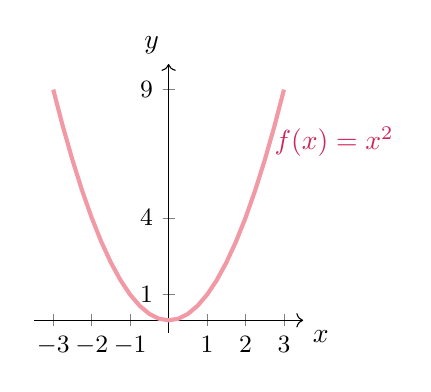
\begin{tikzpicture}[baseline=3cm]
			\begin{axis}[
				clip=false,
				width=5cm, height=5cm,
				xmin=-3.5, xmax=3.5,
				ymin=-0.5, ymax=10,
				xtick={-3,-2,-1,0,1,2,3},
				ytick={1,4,9},
				axis lines=middle,
				axis line style={->},
				xlabel={$x$}, ylabel={$y$},         
				xlabel style={below right},
				ylabel style={above left},
				tick label style={font=\small},
				]
				\addplot[color=pink!80!purple, line width=1.5pt, domain=-3:3] {x^2};
				\node[above right, pink!20!purple] at (2.5, 6) {$f(x)=x^2$};
			\end{axis}
		\end{tikzpicture}
\end{center}
\end{frame}

\begin{frame}
	同样，对于函数$f(x)=-x^2$，你能画出它的图像吗？你能从以它为例说明函数$f(x)$的最大值的含义吗？
	\pause
\begin{center}
	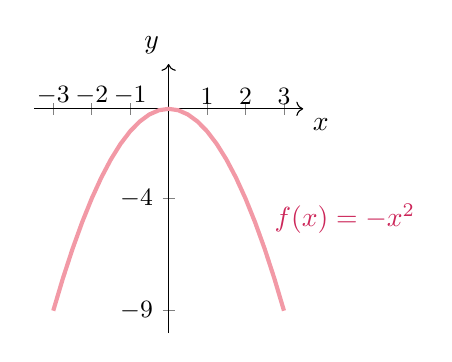
\begin{tikzpicture}[baseline=3cm]
		\begin{axis}[
			clip=false,
			width=5cm, height=5cm,
			xmin=-3.5, xmax=3.5,
			ymin=-10, ymax=2,
			xtick={-3,-2,-1,0,1,2,3},
			ytick={-4,-9},
			xticklabel style={above},
			axis lines=middle,
			axis line style={->},
			xlabel={$x$}, ylabel={$y$},
			xlabel style={below right},
			ylabel style={above left},
			tick label style={font=\small},
			]
			\addplot[color=pink!80!purple, line width=1.5pt, domain=-3:3] {-x^2};
			\node[above right, pink!20!purple] at (2.5, -6) {$f(x)=-x^2$};
		\end{axis}
	\end{tikzpicture}
\end{center}
\end{frame}

\begin{frame}
	\begin{summarybox}[最大值]
		设函数 \(y=f(x)\) 的定义域为 \(D\)，如果存在实数 \(M\) 满足：\\
		(1) \(\forall x\in D\)，都有 \(f(x)\leqslant M\)；\quad (2) \(\exists x_0\in D\)，使得 \(f(x_0)=M\).\\
		那么称 \(M\) 是函数 \(y=f(x)\) 的\textbf{最大值}.
	\end{summarybox}
	
	\pause
	\begin{summarybox-answer}
		\textbf{最小值}：把上述定义中的 \(f(x)\leqslant M\) 改为 \(f(x)\geqslant M\)，其余条件不变，即得最小值的定义.
	\end{summarybox-answer}
\end{frame}

\begin{frame}{例4：烟花爆裂的最佳时刻}
	\setcounter{exam}{3}
	\begin{exam}
	“菊花”烟花冲出后距地面高度 \(h(t)=-4.9t^2+14.7t+18\)（单位：m）. 求烟花冲出后何时是爆裂的最佳时刻，这时距地面高度约为多少（精确到 \(1\,\mathrm{m}\)）？
	\end{exam}
	\pause
	\begin{solve}
	二次函数 \(h(t)=-4.9t^2+14.7t+18\) 开口向下，顶点即最高点.
	

	\[
		t=-\frac{14.7}{2\times(-4.9)}=1.5\ (\mathrm{s}),\qquad
		h=\frac{4\times(-4.9)\times18-14.7^2}{4\times(-4.9)}\approx 29\ (\mathrm{m}).
	\]
	\end{solve}
\end{frame}

\begin{frame}{例4（图）：高度随时间变化}
	\begin{columns}
		\column{0.58\textwidth}
		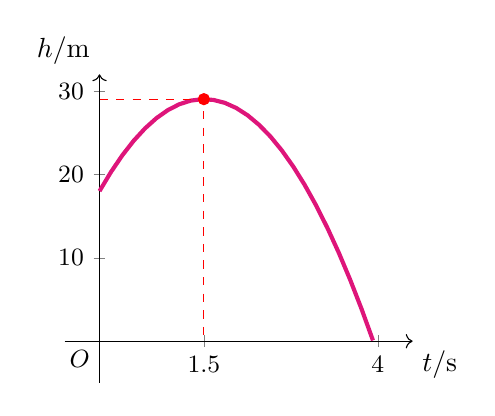
\begin{tikzpicture}[baseline=(current bounding box.north)]
			\begin{axis}[
				width=6cm, height=5.5cm,
				xmin=-0.5, xmax=4.5, ymin=-5, ymax=32,
				xtick={1.5,4},
				ytick={10,20,30},
				axis lines=middle, axis line style={->},
				xlabel={$t$/s}, ylabel={$h$/m},
				xlabel style={below right}, 
				ylabel style={above left},
				tick label style={font=\small},
			]
			\addplot[color=magenta!70!purple, line width=1.5pt, domain=0:3.93] {-4.9*x^2+14.7*x+18};
			\addplot[only marks, mark=*, mark size=2pt, color=red] coordinates {(1.5,29.025)};
			\draw[dashed, red] (0,29.025) -- (1.5,29.025) -- (1.5,0);
			\node[below left] at (axis cs:0,0) {\small$O$};
			\end{axis}
		\end{tikzpicture}
		\column{0.38\textwidth}
		\vspace{2em}
		\begin{summarybox-answer}
		烟花冲出后 \(1.5\,\mathrm{s}\) 是爆裂的最佳时刻，这时距地面高度约为 \(29\,\mathrm{m}\).
		\end{summarybox-answer}
	\end{columns}
\end{frame}

\begin{frame}{例5：求 \(f(x)=\dfrac{2}{x-1}\)，\(x\in[2,6]\) 的最值}
	\begin{exam}
	已知函数 \(f(x)=\dfrac{2}{x-1}\)（\(x\in[2,6]\)），求函数的最大值和最小值.
	\end{exam}
	\pause
	\begin{solve}
	任取 \(x_1,x_2\in[2,6]\)，且 \(x_1<x_2\)，则
	\[
		f(x_1)-f(x_2)=\frac{2}{x_1-1}-\frac{2}{x_2-1}
		=\frac{2(x_2-x_1)}{(x_1-1)(x_2-1)}.
	\]
	由 \(2\leqslant x_1<x_2\leqslant6\)，得 \(x_2-x_1>0,\ (x_1-1)(x_2-1)>0\)，于是 \(f(x_1)-f(x_2)>0\).
	\end{solve}
\end{frame}

\begin{frame}{例5（图）：端点处取得最值}
	\begin{columns}
	\column{0.5\textwidth}
	\hspace{2em}	
	\begin{summarybox-answer}
		所以 \(f(x)=\dfrac{2}{x-1}\) 在 \([2,6]\) 上\textbf{单调递减}.\\[4pt]
		在 \(x=2\) 时取得最大值 \(2\)；在 \(x=6\) 时取得最小值 \(0.4\).
	\end{summarybox-answer}
		\column{0.5\textwidth}
		\vspace{1em}
		\hspace{1cm}
		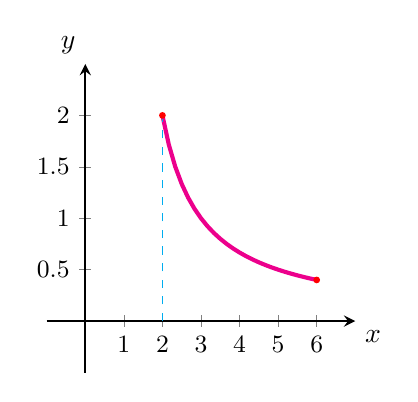
\begin{tikzpicture}[baseline=(current bounding box.north)]
			\begin{axis}[
				width=5.5cm, height=5.5cm,
				xmin=-1, xmax=7, ymin=-0.5, ymax=2.5,
				xtick={1,2,3,4,5,6},
				ytick={0.5,1,1.5,2},
				axis lines=middle, 
				axis line style={-stealth},
				xlabel={$x$}, ylabel={$y$},
				xlabel style={below right}, ylabel style={above left},
				tick label style={font=\small},
				axis line style={thick},
				]
				\addplot[magenta, line width=1.5pt, domain=2:6] {2/(x-1)};
				\addplot[only marks, mark=*, mark size=1pt, color=red] coordinates {(2,2) (6,0.4)};
				\addplot[dashed,cyan] coordinates {(2,0)(2,2)};
			\end{axis}
		\end{tikzpicture}
		
	\end{columns}
\end{frame}

\begin{frame}
	本节课主要内容：
	\begin{enumerate}[(1)]
		\item 最大值
		\item 最小值
	\end{enumerate}
\end{frame}

\begin{frame}
	{布置作业：}
	
	课本P81: 练习 1,2,4\\
	P86 习题4
\end{frame}

\section{课堂练习}

\begin{frame}
	练习 1：整个上午（\(8:00 \sim 12:00\)）天气越来越暖，中午时分（\(12:00 \sim 13:00\)）一场暴风雨使天气骤然凉爽了许多. 暴风雨过后，天气转暖，直到太阳落山（\(18:00\)）才又开始转凉. 画出这一天 \(8:00 \sim 20:00\) 期间气温作为时间函数的一个可能的图象（示意图），并说出所画函数的单调区间.
	
	\begin{solve}
	由题意可知，气温随时间的变化可分为以下几个阶段：
	\begin{itemize}
		\item \(8:00 \sim 12:00\)：天气越来越暖，气温单调递增；
		\item \(12:00 \sim 13:00\)：暴风雨使气温骤降，气温单调递减；
		\item \(13:00 \sim 18:00\)：暴风雨过后转暖，气温单调递增；
		\item \(18:00 \sim 20:00\)：太阳落山开始转凉，气温单调递减。
	\end{itemize}
	所以，该函数在区间 \([8, 12]\) 和 \([13, 18]\) 上单调递增；在区间 \([12, 13]\) 和 \([18, 20]\) 上单调递减。（注：此处的时间单位取为小时）
	\end{solve}
\end{frame}

\begin{frame}
	\begin{center}
		\begin{tikzpicture}
			\begin{axis}[
				width=10cm, height=5.5cm,
				xlabel={时间 \(t\) (小时)},
				ylabel={气温 \(T\)},
				xmin=7.5, xmax=20.5,
				ymin=10, ymax=35,
				xtick={8, 12, 13, 18, 20},
				ytick=\empty,
				axis lines=middle,
				enlargelimits=false,
				clip=false,
				title={气温随时间变化的示意图}
				]
				% 用平滑曲线模拟气温变化
				\addplot [thick, red, smooth] coordinates {
					(8, 16)   % 8:00 较凉
					(10, 22)  % 逐渐升温
					(12, 30)  % 12:00 闷热
					(12.5, 20)% 暴雨中降温
					(13, 16)  % 13:00 骤然凉爽
					(15.5, 24)% 雨后天晴转暖
					(18, 28)  % 18:00 最暖
					(20, 18)  % 20:00 开始转凉
				};
			\end{axis}
		\end{tikzpicture}
	\end{center}
\end{frame}

\begin{frame}
	2.设函数 \(f(x)\) 的定义域为 \([-6, 11]\). 如果 \(f(x)\) 在区间 \([-6, -2]\) 上单调递减，在区间 \([-2, 11]\) 上单调递增，画出 \(f(x)\) 的一个大致的图象，从图象上可以发现 \(f(-2)\) 是函数 \(f(x)\) 的一个 \underline{\hspace{2cm}}(填“最大值”或“最小值”).
	\pause
	\begin{columns}
	\column{0.6\textwidth}
	\begin{solve}
	根据函数单调性的定义：
	在区间 \([-6, -2]\) 上单调递减，意味着图象从左到右呈下降趋势；
	在区间 \([-2, 11]\) 上单调递增，意味着图象从左到右呈上升趋势。
	因此，在 \(x = -2\) 处，函数图象由下降转为上升，形成一个“谷底”。从图象上可以发现，\(f(-2)\) 是函数 \(f(x)\) 的 \textbf{最小值}。
	\end{solve}
	\column{0.4\textwidth}
	
	\vspace{-1em}
		\begin{tikzpicture}[baseline=(current bounding box.north)]
			\begin{axis}[
				width=6cm, height=5.5cm,
				xlabel={\(x\)}, ylabel={\(y\)},
				xmin=-7, xmax=12,
				ymin=-1, ymax=27,
				xtick={-6, -2, 11},
				ytick=\empty,
				axis lines=middle,
				enlargelimits=true,
				clip=false,
				title={\(f(x)\) 的大致图象}
				]
				% 绘制模拟分段单调性的函数图象 (例如一个抛物线)
				\addplot [thick, blue, domain=-6:11, samples=100] {(x+2)^2/8 + 2};
				
				% 标出极小值点
				\addplot [only marks, mark=*, mark size=2pt, red] coordinates {(-2, 2)};
				\node[anchor=south west, text=red] at (axis cs:-2, 2.5) {最小值 \(f(-2)\)};
				
				% 添加辅助虚线
				\draw[dashed, gray] (axis cs:-2,0) -- (axis cs:-2,2);
			\end{axis}
		\end{tikzpicture}

\end{columns}
\end{frame}

\begin{frame}
	\textbf{3.} 已知函数 \(f(x) = \frac{1}{x}\)，求函数在区间 \([2, 6]\) 上的最大值和最小值.
	
	\begin{columns}
		\column{0.6\textwidth}
		\begin{solve}			
			对于任意 \(x_1, x_2 \in [2, 6]\)，且 \(x_1 < x_2\)，有：
			\[
			f(x_1) - f(x_2) = \frac{1}{x_1} - \frac{1}{x_2} = \frac{x_2 - x_1}{x_1 x_2}
			\]
			因为 \(2 \le x_1 < x_2 \le 6\)，所以 \(x_2 - x_1 > 0\)，\(x_1 x_2 > 0\).
			从而 \(f(x_1) - f(x_2) > 0\)，即 \(f(x_1) > f(x_2)\).
			所以函数 \(f(x) = \frac{1}{x}\) 在区间 \([2, 6]\) 上是单调递减函数.
			
			因此：
			当 \(x = 2\) 时，函数取得最大值 \(f(2) = \frac{1}{2}\)；
			当 \(x = 6\) 时，函数取得最小值 \(f(6) = \frac{1}{6}\).
			
		\end{solve}
		\column{0.4\textwidth}
		
		\begin{tikzpicture}
			\begin{axis}[
				clip=false,
				width=5.5cm, height=5.5cm,
				xlabel={\(x\)}, ylabel={\(y\)},
				xmin=0, xmax=7,
				ymin=0, ymax=0.8,
				xtick={2, 6},
				ytick={1/6, 1/2},
				yticklabels={\(\frac{1}{6}\), \(\frac{1}{2}\)},
				axis lines=middle,
				enlargelimits=false,
%				title={\(f(x)=\frac{1}{x}\) 在 \([2, 6]\) 上的图象}
				]
				% 绘制函数图象
				\addplot [thick, blue, domain=2:6, samples=100] {1/x};
				
				% 标记最大值和最小值点
				\addplot [only marks, mark=*, mark size=2pt, red] coordinates {(2, 1/2) (6, 1/6)};
				
				% 添加虚线辅助线
				\draw[dashed, gray] (axis cs:2,0) -- (axis cs:2,1/2);
				\draw[dashed, gray] (axis cs:0,1/2) -- (axis cs:2,1/2);
				\draw[dashed, gray] (axis cs:6,0) -- (axis cs:6,1/6);
				\draw[dashed, gray] (axis cs:0,1/6) -- (axis cs:6,1/6);
				
				% 标注文字
				\node[above right] at (axis cs:2,0.5) {最大值};
				\node[above right] at (axis cs:6,1/6) {最小值};
			\end{axis}
		\end{tikzpicture}
	\end{columns}
\end{frame}


\end{document}
